\documentclass[runningheads]{llncs}

\usepackage{graphicx}
\usepackage{booktabs}
\usepackage{amsmath}
\usepackage{siunitx}

% Package for todo command
\usepackage{xcolor}

\newcommand\todo[1]{\textcolor{red}{#1}}

\begin{document}

\title{My Cool Title}

\author{Jacobus C. Lock\inst{1} \and
  Grzegorz Cielniak\inst{1} \and
  Andrea Tramontano\inst{2} \and
  Nicola Bellotto\inst{1}
}
\authorrunning{J.C. Lock et. al.}
\institute{University of Lincoln, Lincoln, UK \and
  Universita Degli Studi Di Padova, Italy
}

\maketitle

\begin{abstract}
  Cool abstract here
  \keywords{All the best keywords}
\end{abstract}

\section{Introduction}

It is estimated that there are almost half a billion people today that live with mild to severe levels of vision impairments or total blindness and this number is expected to significantly rise with an ageing population~\cite{bourne2017magnitude}.
There has been a rise interest from industrial partners in utilising modern technology to make their products more accessible and improvements in modern computing power and image processing capabilities have made this easier.
The work we present here is part of the ActiVis project that aims to assist people with vision impairments (PwVI) to independently navigate and find objects within an unknown indoor environment using only a mobile phone and its camera.
This system implements ideas from the active vision field~\cite{bajcsy2017,bellotto2013}, but replaces the electro-mechanical servo typically found in active vision systems, with a user's arm and hand as pictured in Fig.~\ref{fig:system-in-use}\todo{replace with actual picture}.
This project expands upon concepts originally proposed in~\cite{bellotto2013} and~\cite{lock2017portable} and builds off of the system introduced in~\cite{lock2019active}.

\begin{figure}
  \centering
  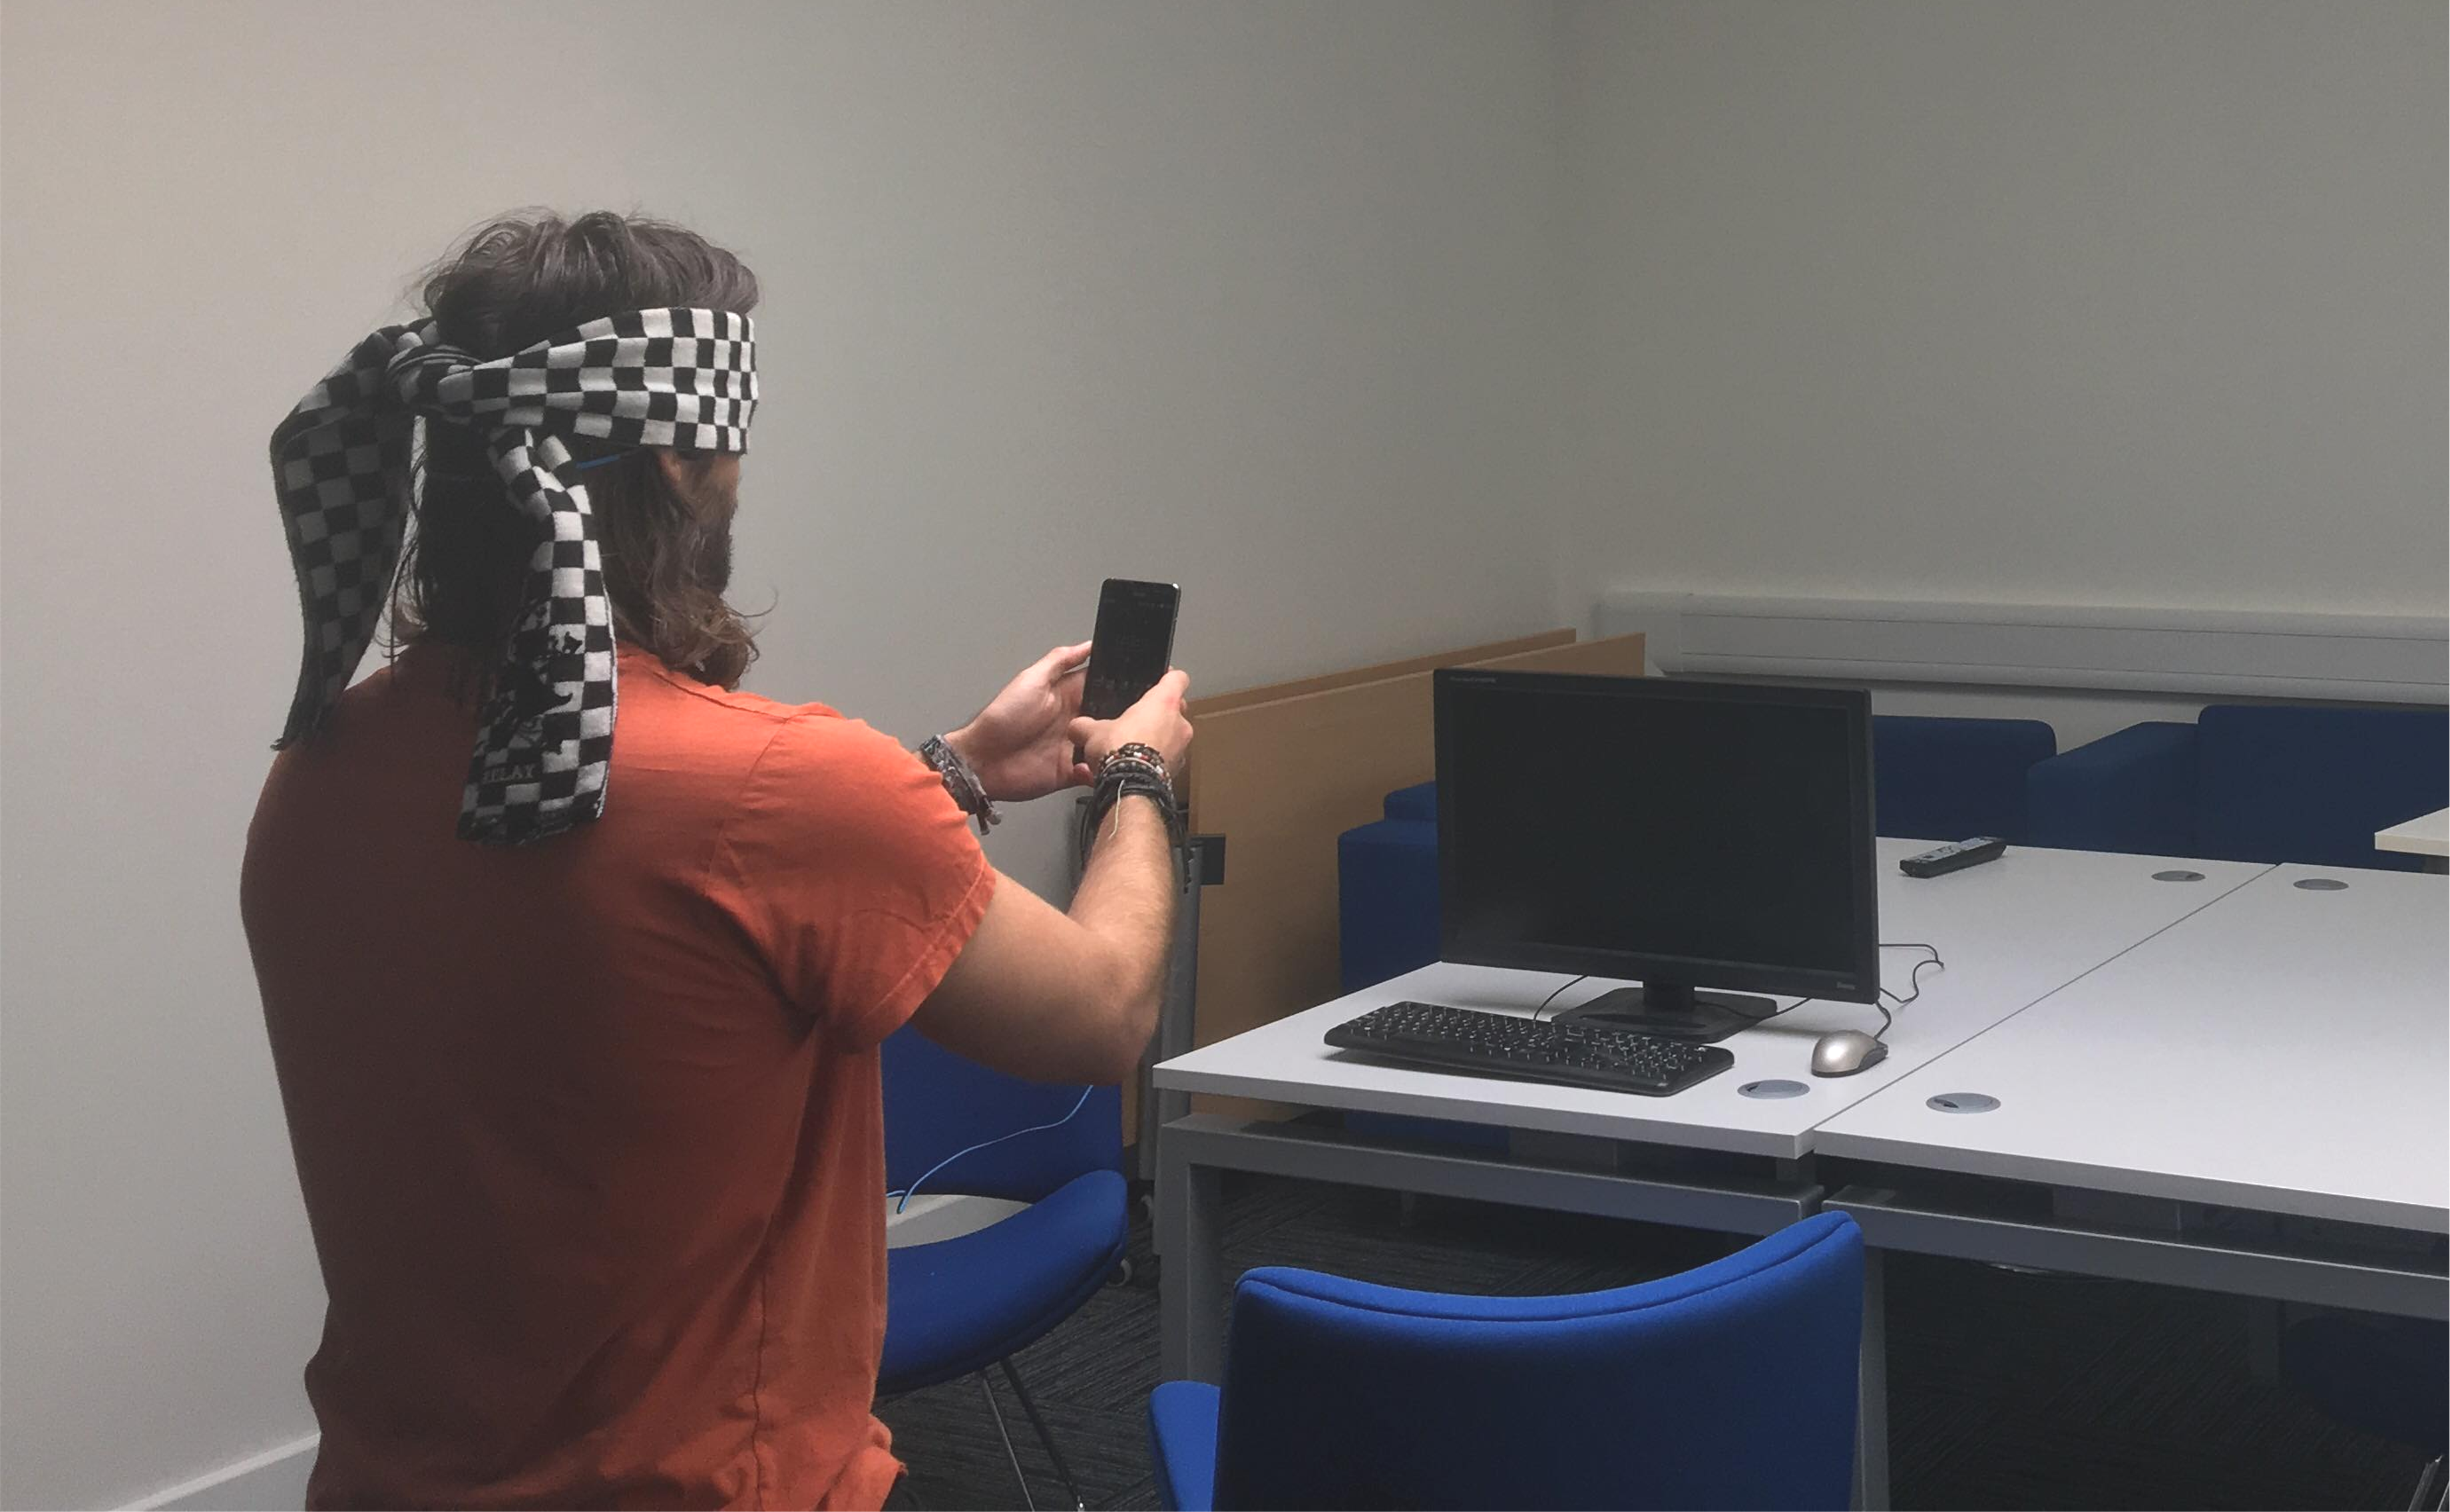
\includegraphics[width=0.5\textwidth]{figures/system_use.png}
  \caption{The system in use during an experiment. }\label{fig:system-in-use}
\end{figure}

Our active search system uses the camera's current and previous views as input and leverages its understanding of inter-object spatial relationships to determine the best navigation action to determine the best action to take to reach the target object.
To enable this, we expanded upon our previous work and implemented a partially observable Markov Decision Process (POMDP)~\cite{bellman1957markovian} on a mobile phone generates real-time navigation instructions to guide the user to their target object.

This work includes the following contributions:

\begin{itemize}
  \item a POMDP-based human controller that enables object search and guidance on a mobile phone;
  \item a complete system pipeline that includes guidance instruction generation and transmission;
  \item experiments that evaluate the efficacy of the proposed system.
\end{itemize}

Section~\ref{sec:previous-work} discusses relevant work that has already been done, followed by a description of the active vision system and human controller in Sections~\ref{sec:active-vision} and~\ref{sec:human-controller} respectively. 
The experiments that were conducted in this work, and their results, are discussed in Sections~\ref{sec:experiments} and~\ref{sec:results}, followed finally by a short conclusion and discussion of the next steps for the project in Section~\ref{sec:conclusion}.

\section{Previous Work}\label{sec:previous-work}

\section{Active Vision System}\label{sec:active-vision}

The work we present in this paper is an advancement towards the ActiVis projects larger goal of developing a stand-alone mobile system that can guide a PwVI towards their desired destination with minimal user input or intervention. 
This work focuses on guiding a user towards an object in one, static environment and is limited to 2 dimensions (pan and tilt).

A complete system diagram is given in Fig.~\ref{fig:sys-diagram}\todo{cite own work where fig is from if necessary}. 
This diagram shows a typical feedback control loop that generates a control signal to minimise some error signal, but has been modified to incorporate a human within the loop.

\begin{figure}
  \centering
  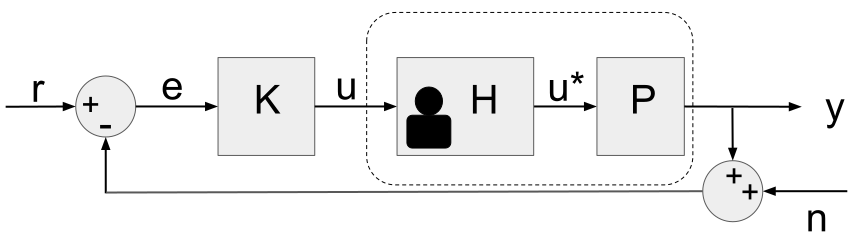
\includegraphics[width=0.75\textwidth]{figures/control_loop.png}
  \caption{System control loop: $r$ is the reference object, $e$ the error signal, $u$ and $u^*$ the original and interpreted control signals and $y$ is the current object observation. $K$, $H$ and $P$ are the control, human and sensor blocks respectively. }\label{fig:sys-diagram}
\end{figure}

In this case, the error is defined as the difference between the desired object and the object currently within view. 
The implication of this modification is that an additional block, \emph{H}, is added to simulate a human that receives an control signal, \emph{u}, from the controller, \emph{K}. 
However, the challenge with people is that a person may interpret \emph{u} in any unpredictable way (i.e.\ apply a transformation) that results in the signal \emph{u*} that points the camera, \emph{P}, to a new location containing a new object observation, \emph{y}.
It is therefore important to design \emph{K} to take be robust enough to accommodate different user habits and limitations and ensure that \emph{u*} tracks \emph{u} as closely as possible. 
These design considerations are addressed in previous work. \todo{how to state that we designed the interface already if its unpublished?}

Another fact to take note of is the measurement noise, \emph{n}, added in the feedback loop that simulates an object detector making classification errors that will influence the action that \emph{K} generates. 
In our previous work, we assumed a `perfect classifier' and solved the problem using a plain Markov decision process (MDP). 
In this work we do away with that somewhat naive assumption and implement a POMDP that can better handle the observation uncertainties inherent to modern object detectors and classifiers. 
The design of the human controller is discussed next. 

\section{Human Controller}\label{sec:human-controller}

The POMDP human control module that we implemented for this work is an extension to the MDP-based controller we made for the experiments described in~\cite{lock2019active}.
It works by generating a trail of virtual waypoints for the user to point the camera towards.
The waypoint positions are based on the model's pre-trained, internal knowledge on the inter-object spatial relationships and they are placed in a way that maximises the probability of the user pointing to and finding the target object
A new waypoint is generated when the user finds the current waypoint or finds another ancillary object.
The design and implementation of this POMDP human controller is discussed here.

\subsection{Design}

A POMDP is an extension to the MDP model that allows it to handle cases where the state is not directly observable, allowing it to be used in more realistic scenarios. 
In this case, the state is inferred based on the model parameters and the associated sensor accuracy (if a sensor is 100\% accurate, the state would be directly observable).
The implication of this is that a POMDP-based agent does not know its state at any point in time.
Instead, a POMDP model relies on a so-called belief meta-state that changes with additional observations to reflect the likelihood the agent is in any given state.
The belief state is fully observable by the agent and can be used to infer the parent POMDP-agent's current state and generate the next action, hence the designation as an MDP.\@

The system uses an object detector and classifier in order to find any objects within the camera's view.
These detectors and classifiers have some noise associated with them that is caused by misclassifications and similar errors and a POMDP is therefore necessary in this case.

A POMDP model is represented by the $n$-tuple

\begin{equation}
  (\mathbf{S}, \mathbf{A}, \mathbf{T}, \mathbf{R}, \mathbf{\Omega}, \mathbf{O}, \mathbf{b}, \gamma),
\end{equation}

\noindent where $\mathbf{S}$ represents a finite set of discrete states, $\mathbf{A}$ is a set of discrete actions the agent can execute in any state, $\mathbf{T}$ is a matrix containing the probabilities of transitioning from state $s$ to state $s'$, $s, s' \in \mathbf{S}$ after executing action $a$, $a \in \mathbf{A}$ and $\mathbf{R}$ is the reward the agent receives for reaching state $s'$ after executing action $a$.
$\mathbf{\Omega}$ is a set of possible state observations the agent can make, while the table $\mathbf{O}$ contains the probabilities of making state observation $\omega$, $\omega \in \mathbf{\Omega}$, when in state $s$ after executing action $a$.
Finally, $\mathbf{b}$ is the belief vector containing the state probability distribution and the scalar $\gamma$ is a discount factor that prioritises long-term over short-term rewards and affects the model's convergence rate. 
The belief state $\mathbf{b}$ is updated for every timestep and action-observation pair.
This update is done with

\begin{equation}
  b_t(s') = \eta\Omega(o, s', a)\sum_{s\in\mathbf{S}}\mathbf{T}(s, a, s')b_{t-1}(s)
\end{equation}

The state and space spaces and the reward and transition functions for this POMDP are the same as the MDP described in~\cite{lock2019active}. 
The major difference is the addition of an observation matrix that defines the probability of being in any given state after making a new observation.
In essence, it is a measure of the sensor accuracy, and in this case it describes the object detector's classification accuracy and recall.
These parameters are given by the following. 

\subsubsection{State Space}

The state is given by

\begin{equation}
  s = \langle z, n, v \rangle,
\end{equation}

\noindent where $z, z\in\mathbf{z}$, is the object within view, n the number of search steps taken since the search began and a binary variable $v$ that tracks the uniqueness of a waypoint's position for the search.

\subsubsection{Actions}

The possible actions an that define the area where the agent will generate the next waypoint are given by

\begin{equation}
  \mathbf{A} = \{ \textrm{UP, DOWN, LEFT, RIGHT} \}
\end{equation}

\subsubsection{Transitions}

$\mathbf{T}$ was determined by extracting the inter-object spatial relationships for the objects of interest in terms of the actions in $\mathbf{A}$ from the OpenImages\todo{cite} dataset. 
For example, by iterating over all of the images containing the objects of interest, we can see that the object `monitor' is located above (i.e. UP) the object `keyboard' in 87\% \todo{get real percentage} of images containing both objects. 
The transition function for this case will look like 

\begin{equation}
  \mathbf{T}(s, a, s') = \mathbf{T}(\textrm{keyboard}, \textrm{UP}, \textrm{monitor}) = 0.87
\end{equation}
An example of this relationship can be seen in the image in Fig.~\ref{fig:openimage}.

\begin{figure}
  \centering
  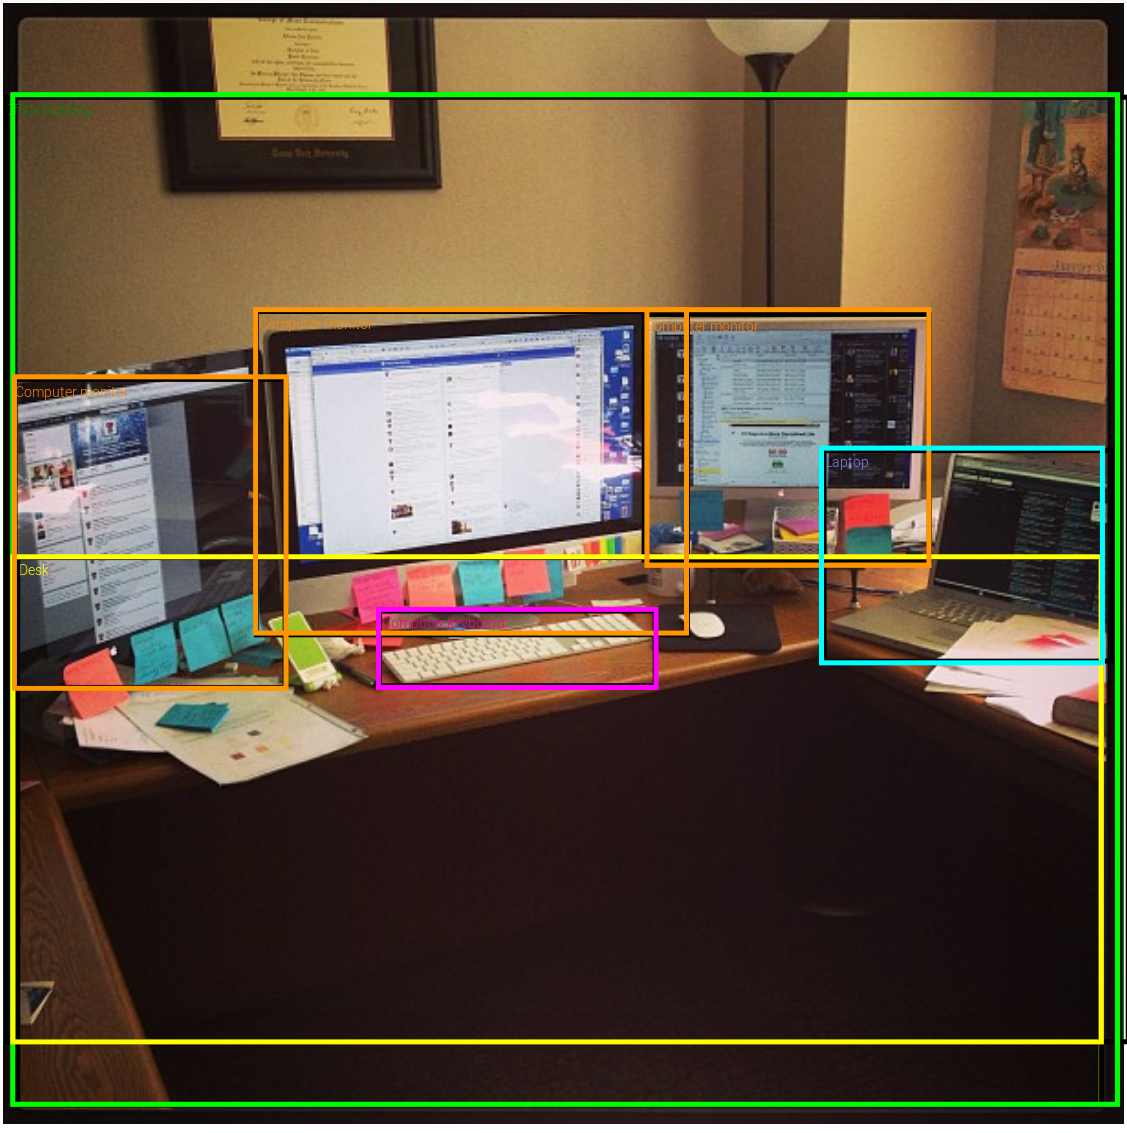
\includegraphics[width=0.5\columnwidth]{figures/desk_example.png}
  \caption{}\label{fig:openimage}
\end{figure}

\subsubsection{Reward Function}

The reward function is designed to encourage the agent to find the target object by giving it a substantial reward for doing so, while penalising it for every action it takes that does not results in it finding the target object.
Furthermore, additional penalties are given if the agent generates a waypoint in an area it has explored before $(v = \textrm{true}$) and when it exceeds some search length threshold, denoted by $n_{\max}$.
All of the rewards and when they are given are summarised by Table~\ref{tab:rewards}.

\begin{table}
  \centering
  \caption{The reward function for the POMDP. }\label{tab:rewards}
  \begin{tabular}{cc}
    \toprule
    $r(o = o_{target})$ & 10000 \\ \midrule
    $r(v = \textrm{true})$  & -75 \\ \midrule
    $r(n > n_{\max})$ & -75 \\ \midrule
    otherwise $r(\cdot)$ & -100  \\ \midrule
    \bottomrule
  \end{tabular}
\end{table}

\subsubsection{Observations and Observation Matrix}

The observations the agent can make are identical to the states that the agent can enter. 
In this case, however, the only uncertainty in the system is introduced by the object detector, since the model can perfectly track the number of steps taken during the search and the locations that waypoints have been generated.
$\mathbf{\Omega}$ therefore only contains the classification/misclassification probabilities of the object detector. 
These values were found by performing a set of classifier tests on the object detector and generating a confusion matrix to populate $\mathbf{\Omega}$.

\subsubsection{Training}

For our system, we encoded a total of 16 objects, including a `nothing' state where the detector does not see anything of interest, into the POMDP and object detector. These objects are given by $\mathbf{z}$, defined as 

\begin{equation}
  \begin{split}
    \mathbf{z} = \{ nothing, monitor, keyboard, mouse, desk, laptop, mug, window,\\ 
      lamp, backpack, chair, couch, plant, telephone, whiteboard, door \}
  \end{split}
\end{equation}

We also set $n_{\max}$ to 12 waypoints, after which the agent gets penalised for every additional waypoint it generates that does not lead to the target object. 
This results in a total of 352 reachable states ($n_{states} = 16\times11\times2$), with any state containing the target object acting as a terminal state.

The POMDP model is put through a training process to generate a policy that contains the optimal belief-action mapping that an agent can use to produce the optimal waypoint locations.
This is done by having the agent explore the entire state-action-observation space and optimising the policy to maximise the long-term cumulative reward.

The difficulty of solving POMDPs is that the belief vector is a vector of continuous probability distributions with infinite combinations, making them very time-consuming or even impossible to solve exactly and we found this to be the case for our moderately-sized state space size and therefore opted to use an approximate method instead.
Multiple algorithms that solve POMDPs approximately have been proposed\todo{cite examples} and in this work we used the Point-Based Value Iteration (PBVI) algorithm~\cite{pineau2003point} to solve the POMDP model.
The PBVI algorithm speeds up the optimisation process by selecting a smaller subset of representative belief points from the belief function and tracking the values and derivatives of those points only. 
Using the PBVI algorithm, we generated a total of 15 policies, one for each target object. 

\subsection{Controller Implementation}

We made an Android app that implements the object detector and POMDP controller onto a mobile phone that can generate and provide guidance instructions for a user.  
This was done by combining an audio interface that can provide non-visual guidance instructions, the POMDP controller and object detector onto a mobile app.
Each of these aspects and their implementation are discussed here.

\subsubsection{Audio Interface}

The target audience of our system are PwVI and we therefore have to provide guidance instructions in a non-visual manner that is intuitive and easy to understand. 
To avoid blocking a user's access to the ambient sounds (something PwVI typically rely upon extensively), we use a set of non-intrusive bone-conducting headsets to transmit the audio signals to the user. 

To describe the waypoints pan and tilt positions, we implemented an improved version of the interface described in~\cite{bellotto2013} that uses a spatialised audio signal.
However, in this work we only spatialise the audio in the pan dimension only, since our headphones bypass the ear's pinnae that allow a person to determine the tilt angle of a sound source. 
Instead we exploit a human's natural association of high and low sound sources with a high and low sound frequency respectively~\cite{blauert1997spatial} and adjust the sound source's pitch as a function of the waypoint's tilt angle. 
A similar interface was used in~\cite{schauerte2012assistive}.
With this interface and set of headphones, we are able to describe the location of a waypoint to a user in 2 dimensions (pan and tilt) in an intuitive an non-intrusive manner. 

\subsubsection{Object Detector}

\subsubsection{POMDP Controller}

The output from the POMDP model's training process is a policy file that defines the best location to place the next search waypoint based on the device's current state.
This state is tracked by the device during run-time by recording the device's previous search locations and previous waypoint positions, which is done by disretising the world into a $6\times6$ grid and setting the relevant grid unit's $v$ value.
Each grid square represents a \SI{35}{\degree} angular translation, encompassing a \SI{210}{\degree}$\times$\SI{210}{\degree} field of view. 
This setup gives the state access to perfectly observable $n$ and $v$ parameters, while the observation parameter $o$ is generated by the object detector. 

When the user moves the device into a new grid square by rotating the device past \SI{35}{\degree}, thereby making a new $v$ observation and changing the state, or observes a new object, the device triggers the controller to generate a new waypoint location.
The controller uses the new state observation $\omega$ to update its belief state and queries the policy for the best location to place the new waypoint. 
The policy output is an action from the action set $\mathbf{A}$ that specifies the next adjacent grid square to place the waypoint.
For example, an `UP' output would result in the waypoint being placed one grid square, i.e. \SI{35}{\degree}, above where the current grid square within view. 

\section{Experiment Design}\label{sec:experiments}

To evaluate the effectiveness of our POMDP controller and guidance system, we designed a set of experiments that can measure its performance in driving a user towards a target object within the environment. 
We also conducted an additional set of experiments with an alternative guidance system to act as a baseline measurement to compare our results to and provide additional context. 
This alternative `guidance' system does not actually provide any guidance instructions to the user, instead it provides the user with the raw observation output from the object classifier and makes use of the user's intuition and prior environment knowledge to generate actions. 
The goal of both the guided and unguided experiment cases were to find an object within a static environment. 

We recruited 10 sighted participants that were blindfolded for the experiments, as well as 2 legally blind participants, where 1 was blind from birth and the other suffers from late onset blindness\todo{Give participant stats}.
Details on the design of these experiments are given in the next sections. 

\subsection{Unguided Case}

The design goal of this experiment is to mimic how a typical person with healthy eyesight would behave if told to look for a given object. 
In such a scenario, a person would exploit the objects currently within their view and their prior knowledge on a room's typical layout to make a decision on where to look next to find what they are looking for. 
Take for example a person in bathroom facing the basin after washing their hands and looking for a hand-dryer. 
It is unlikely that a hand dryer would be placed above or below a wash basin so it it is reasonable to believe that they would instinctively look at chest height on the walls to their left, right or behind them to find a dryer. 

For this experiment, a mobile camera and object detector acts as the participant's eyes and informs them what the objects within the camera's view and it is then up to the participant to exploit their prior knowledge of the given environment in order to manipulate the camera to point towards the target object. 
This process is modelled by the schematic in Fig.~\ref{fig:sys-diagram-no-controller}, \emph{H}, acts as both the actuator and controller.
The object detector was implemented in an Android app that uses the object classifier and Android's Text-to-Speech engine to read out any objects that it detected. 
The app only reads out the objects when the participant requested it to by tapping on the screen. 
When the target object comes within the camera's view and is correctly classified by the object detector, the device vibrated to inform the participant. 

\begin{figure}
  \centering
  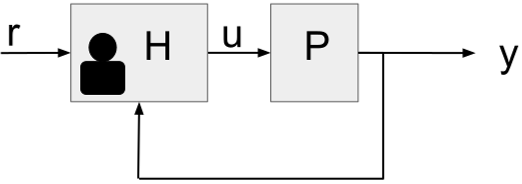
\includegraphics[width=0.7\textwidth]{figures/control_loop_no_controller.png}
  \caption{A set of CDFs comparing the time to target. }\label{fig:sys-diagram-no-controller}
\end{figure}

Each participant was verbally told what the target object was they they were meant to find and each participant was given 45 seconds to find the target object. 
In this case, the learning effect was ignored in order to mimic the typical search behaviour described earlier. 
Each experiment run was ended when a target was found or the time limit was reached. 
This process was repeated a total of 8 times, once for each target object within the environment. 

\subsection{Guided Case}

In this experiment, we evaluate the performance of the guidance system in the object search task, where the perception and control tasks are performed by the guidance system and mobile device and the participant acts as the actuator, interpreting control signals and outputting actuation forces on the camera sensor. 
This is modelled by the schematic in Fig.~\ref{fig:sys-diagram}. 

The participants were not told what the targets objects were in this experiment to eliminate the possibility of them ignoring the guidance instructions in order to try and find the target object themselves.
An experiment run was therefore initiated when the experiment staff selected the target and was terminated when the target object was found or the time limit was exceeded.
We set a time limit of 45 seconds in this experiment as well.
Each participant repeated this experiment 8 times, once for each object within the experiment's object set. 

\subsection{Environment Setup}

The environment, and the object placement within it, for both experiments was modelled on a typical office.
Measures were taken to ensure that both office environments were unique in layout and object placement. 
However, for the larger, more static objects (e.g.\ a desk or door) there is cross-experiment occurrences, since most offices contain the same basic furniture and objects. 
These objects were placed in different locations relative to each other for the 2 experiments to minimise any learning effects that may occur between the experiments. 
All of the objects and their experiment placement is given in Table~\ref{tab:objects}.

\begin{table}
  \centering
  \caption{The different objects used within each experiment environment.}\label{tab:objects}
  \begin{tabular}{p{2cm}cp{0.7cm}c}
    \toprule
    & \bf{Guided} & & \bf{Unguided} \\\midrule
    Door        & X & & X \\\midrule
    Desk	& X & & X \\\midrule
    Chair	& X & & X \\\midrule
    Whiteboard	& X & & X \\\midrule
    Mouse	& X & & X \\\midrule
    Monitor	&   & & X \\\midrule
    Telephone	&   & & X \\\midrule
    Keyboard	&   & & X \\\midrule
    Laptop	& X & &   \\\midrule
    Backpack	& X & &   \\\midrule
    Mug		& X & &   \\\midrule
    \bottomrule
  \end{tabular}
\end{table}

\section{Results}\label{sec:results}

\subsection{Time to Target}

The time it took a participant to find a target object is an important indicator of performance for the system, where less time indicates a shorter search time and increased performance.
The data for the search times for each dataset are given in Fig~\ref{fig:boxplot-time}, while Fig.~\ref{fig:cum-time} shows the cumulative distribution functions (CDF) for the search times as a function of the total number of objects found.

\begin{figure}
  \centering
  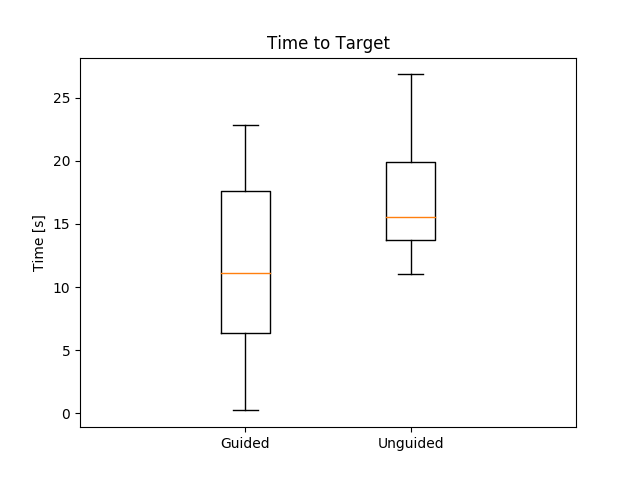
\includegraphics[width=0.7\textwidth]{figures/boxplot_time_to_target.png}
  \caption{A set of boxplots comparing the time to target. }\label{fig:boxplot-time}
\end{figure}

\begin{figure}
  \centering
  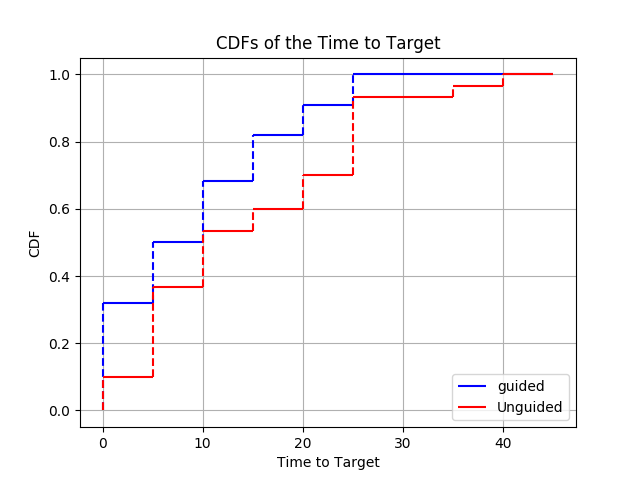
\includegraphics[width=0.7\textwidth]{figures/cumplot_time_to_target.png}
  \caption{A set of CDFs comparing the time to target. }\label{fig:cum-time}
\end{figure}

By inspecting the boxplots in Fig.~\ref{fig:boxplot-time}, it can be seen that the guidance system reduced the time it took the participants to find the targets on average from 17.8s to 10s per target, ($p = 0.038$).
This is an average improvement of almost 40\%.
This is supported by the CDFs in Fig.~\ref{fig:cum-time} that show that \todo{Discuss the less number of objects found and how it is not statistically signioficatn. Perhaps show it in CDF}

\subsection{Movement}

To give an indication of the effort required to find each target, we look at the mobile device's displacement data. 
In this case, less device displacement is desirable, since it implies less physical exertion was demanded from the user, enhancing the user experience\todo{maybe cite paper that says less exertion is good}.

The device displacement was both linear and angular in the $x, y, z, \phi$ (pan) and $\theta$ dimensions.
By integrating these data with respect to time, we can get the total displacement for each dimension.

\section{Conclusion}\label{sec:conclusion}

\bibliographystyle{splncs04}
\bibliography{bib}

\end{document}
